\chapter{Θεωρητικό Υπόβαθρο}

Στο παρόν κεφάλαιο θα οικοδομήσουμε την απαραίτητη γνώση στην οποία βασίζεται η έρευνα των επόμενων ενοτήτων. Αρχικά, θα παρουσιαστούν συνοπτικά τα τεχνητά νευρωνικά δίκτυα \footnote{Από εδώ και στο εξής, με τον όρο \textquote{νευρωνικά δίκτυα} θα αναφερόμαστε στα \textquote{τεχνητά νευρωνικά δίκτυα}.} υπό μια μαθηματική σκοπιά. Έπειτα, θα αναλυθούν τα \hyperlink{_capsule_networks}{νευρωνικά δίκτυα με κάψουλες} (\hyperlink{_capsule_networks}{\en{capsule networks}}) τα οποία και αποτελούν το κύριο θέμα της εργασίας. Τέλος, θα γίνει αναφορά σε νέες τεχνικές και αλγορίθμους που χρησιμοποιήθηκαν στο παρόν έργο ώστε η μετέπειτα εισαγωγή των μεθόδων μας για την εξέλιξη των νευρωνικών δικτύων με κάψουλες να είναι περισσότερο ομαλή και κατανοητή.

\section{Τεχνητά Νευρωνικά Δίκτυα}
Τα σημερινά τεχνητά νευρωνικά δίκτυα, όπως είναι αναμενόμενο, απέχουν σημαντικά από το πρώτο μοντέλο των \en{Warren McCulloch} και \en{Walter Pitts} \cite{mcculloch1943logical} που συζητήσαμε στην ενότητα \ref{historic_note}. Με την ωρίμανση της τεχνολογίας, αυτή ανεξαρτητοποιήθηκε από την \hyperlink{_computational_neuroscience}{(υπολογιστική) νευροεπιστήμη} και εντάχθηκε στην Τεχνητή Νοημοσύνη υπό μια ιεραρχική δομή. Κρίνεται λοιπόν σκόπιμο να παρουσιάσουμε αυτήν την ιεραρχική δομή οργάνωσης της Τεχνητής Νοημοσύνης και μετέπειτα να αναφερθούμε στα επιμέρους στοιχεία της.
\par

\begin{figure}[h]
    \centering
    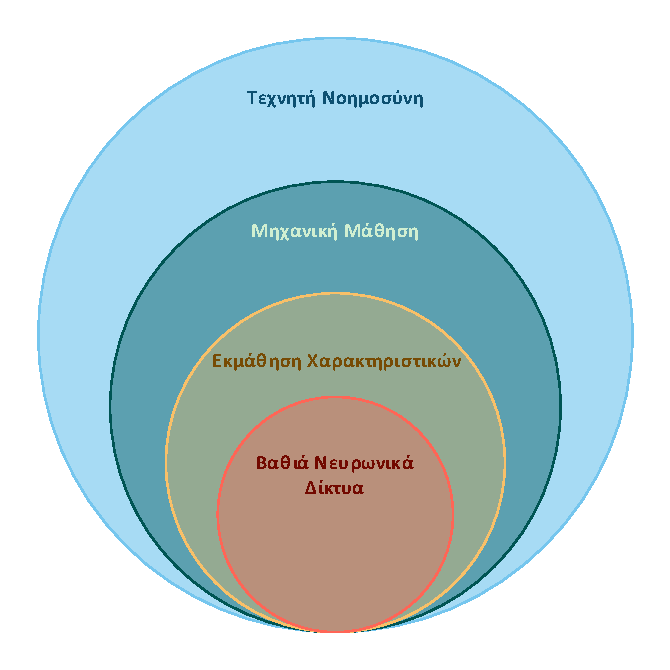
\includegraphics[width=0.7\textwidth]{images/chapter theoritical background/venn ai diagram thesis in greek new 2.pdf}
    \caption{Διάγραμμα \en{Venn} όπου απεικονίζει τη θέση των νευρωνικών δικτύων στην οργάνωση της τεχνητής νοημοσύνης. \textit{Παράχθηκε από το \href{https://www.microsoft.com/en-gb/microsoft-365/visio/flowchart-software/}{\en{Microsoft Visio\texttrademark}.}} }
    \label{fig:_venn_ai}
\end{figure}

Όπως βλέπουμε στο σχήμα \ref{fig:_venn_ai} τα νευρωνικά δίκτυα πολλών επιπέδων (βαθιά νευρωνικά δίκτυα) είναι ένα μέρος του κλάδου της εκμάθησης χαρακτηριστικών (\en{feature learning} ή \en{representation learning}) που είναι ένα μέρος της μηχανικής μάθησης η οποία με τη σειρά της ανήκει στο ευρύτερο επιστημονικό πεδίο της τεχνητής νοημοσύνης. Φυσικά, η τεχνητή νοημοσύνη περιλαμβάνει αρκετούς άλλους κλάδους εκτός από αυτόν της μηχανικής μάθησης\footnote{Βέβαια, ο κλάδος της μηχανικής μάθησης είναι σήμερα ο γρηγορότερα αναπτυσσόμενος.}. Μια χρήσιμη παρατήρηση είναι ότι οι σχέσεις υποσυνόλου συμπίπτουν με τη χρονική αλληλουχία ανάπτυξης του κάθε κλάδου. Δηλαδή, κάθε υποσύνολο αναπτύχθηκε ταυτόχρονα ή αργότερα από το οποιοδήποτε υπερσύνολό του.
\par
Στη συνέχεια, θα γίνει λόγος για τα στοιχεία εκείνα που περιλαμβάνουν την τεχνολογία των βαθιών νευρωνικών δικτύων προκειμένου ο αναγνώστης να αποκτήσει μια εποπτικότερη εικόνα.

\subsection{Μηχανική Μάθηση}


Όπως προδίδει ο όρος, σε αδρές γραμμές τα συστήματα μηχανικής μάθησης έχουν τη δυνατότητα να μαθαίνουν μια εργασία χωρίς να έχουν προγραμματιστεί με ρητές εντολές για τη συγκεκριμένη εργασία αυτή\footnote{Η δυνατότητα αυτή είναι πολύ σημαντική αφού, όπως διαπιστώσαμε στην ενότητα \ref{sec:historic_note} όταν έγινε λόγος για τα έμπειρα συστήματα, για πολλές εργασίες είναι πρακτικός αδύνατο να περιγραφούν ρητά και ντετερμινιστικά οι λύσεις τους.}. Ίσως, ο πιο πλήρης ορισμός δίνεται από τον \en{Tom M. Mitchell} \cite{mitchell1997machine} σύμφωνα με τον οποίο, ένα υπολογιστικό πρόγραμμα λέγεται ότι μαθαίνει από μια εμπειρία \en{E}, ως προς ένα σύνολο εργασιών \en{T} και ένα μέτρο απόδοσης \en{P}, εάν η απόδοσή του σε εργασίες του \en{T}, όπως αυτή μετριέται από το \en{P}, βελτιώνεται με την \en{E}. \footnote{Ο ορισμός αυτός εξηγεί γιατί για παράδειγμα η λήψη μιας ιστοσελίδας της βικιπέδιας και η αποθήκευσή της τοπικά στον υπολογιστή δεν αποτελεί μηχανική μάθηση. Όπως προκύπτει, η \textquote{γνώση} αυτή δεν καθιστά καλύτερο τον υπολογιστή σε κάποια εργασία\cite{geron2019hands}.}
\par

Σύμφωνα με τον ανωτέρω ορισμό διακρίνουμε τρία βασικά συστατικά ενός συστήματος μηχανικής μάθησης. Αυτά είναι τα παρακάτω:
\begin{description}
\item [Εργασία - \en{T}] Είναι το πρόβλημα το οποίο επιθυμούμε να λύσουμε.
\item [Μέτρο Απόδοσης - \en{P}] Αποτελεί μια μετρική του στόχου ως ένδειξη ποιότητας της λύσης μας. Από μαθηματική σκοπιά, είναι αυτό που ο αλγόριθμος μάθησης βελτιστοποιεί.
\item [Εμπειρία - \en{E}] Πρόκειται για τα δεδομένα εισόδου που λαμβάνει το σύστημα υπό τη μορφή παραδειγμάτων ή ως ερεθίσματα ανάδρασης από το περιβάλλον. Όπως θα δούμε στη συνέχεια, ο τρόπος απόκτησης αυτών των δεδομένων αλλά και η φύση τους καθορίζει το είδος της μάθησης.
\end{description}

\subsubsection{Βασικά Είδη Συστημάτων Μηχανικής Μάθησης}
Τα είδη των συστημάτων μηχανικής μάθησης μπορούν να ταξινομηθούν ανάλογα με το:
\begin{itemize}
    \item \emph{Αν εκπαιδεύονται με ανθρώπινη επίβλεψη.}\\
    Ανάλογα με αυτό το κριτήριο έχουμε τις εξής βασικές κατηγορίες: επιβλεπόμενη (\en{supervised}), μη-επιβλεπόμενη (\en{un-supervised}) και ενισχυτική μάθηση (\en{reinforcement learning}).
    \item \emph{Αν μαθαίνουν σταδιακά (\en{incrementally}) και \textquote{στον αέρα} (\en{on the fly}).}\\
    Σε αυτήν την περίπτωση χωρίζουμε τα συστήματα μηχανικής μάθησης σε αυτά που πραγματοποιούν μάθηση σε ζωντανό χρόνο (\en{online learning}) και σε αυτά που μαθαίνουν κατά δέσμες (\en{batch learning}).
    \item \emph{Αν κατασκευάζουν μοντέλα προσαρμοσμένα στα δεδομένα.}\\ 
    Με αυτό το κριτήριο χωρίζονται σε συστήματα βασισμένα σε μοντέλο (\en{model-based}) ή σε συστήματα βασισμένα σε παραδείγματα (\en{instance-based}). \cite{geron2019hands}
\end{itemize}

Προφανώς, κάθε δυνατός συνδυασμός των παραπάνω κριτηρίων είναι αποδεκτός, οδηγώντας έτσι στην ταξινόμηση των συστημάτων μηχανικής μάθησης σε μια πληθώρα από διαφορετικές κατηγορίες. Κρίνεται χρήσιμο, να αναφέρουμε σε όλη την έκταση του έργου τις κατηγορίες στις οποίες ανήκει το κάθε σύστημα που παρουσιάζουμε. Για αυτόν τον λόγο, παροτρύνουμε τον αναγνώστη που δεν είναι εξοικειωμένος με τους ανωτέρω όρους να διαβάσει τους αντίστοιχους ορισμούς στο παράρτημα \ref{chap:definitions}. 
\subsection{Εκμάθηση Χαρακτηριστικών}
 
\subsection{Πολυεπίπεδα Νευρωνικά Δίκτυα}
Η ανάπτυξη των πρώτων συστημάτων μηχανικής μάθησης απεμπόλησε την ανάγκη των ευφυών εφαρμογών για σχολαστική και ρητή (\en{hard-coded}) αναπαράσταση του χώρου του προβλήματος (μιας και αυτή αποκτιούνταν πλέον με αυτοματοποιημένο τρόπο). Με τα νέα συστήματα, ο χώρος του προβλήματος μαθαίνονταν μέσω αλγορίθμων μάθησης από το σύνολο δεδομένων εκπαίδευσης.
\label{sec:_vanilla_nn}
\subsection{Συνελικτικά Νευρωνικά Δίκτυα}
\subsection{Εκπαίδευση Νευρωνικών Δικτύων}
\subsection{Στρατηγικές Βελτίωσης Απόδοσης Νευρωνικών Δικτύων}
\section{Νευρωνικά Δίκτυα με Κάψουλες}
\section{Μηχανισμός Προσοχής}
\section{Μετασχηματιστές}
\section{Χάρτες Αυτο-οργάνωσης}
\label{sec:_SOM}
\section{Αλγόριθμος \en{EM}}
\label{sec:_EM}
\section{Συμπερασματολογία μέσω Διακύμανσης}
% autoencoders